\section{Theory of personal information}
\begin{center}
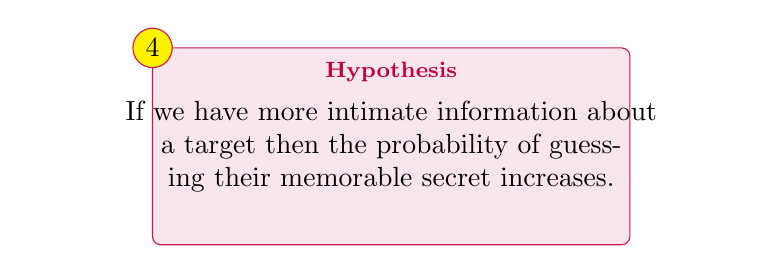
\begin{tikzpicture}
    \def\gridwidth{0.5\textwidth}
    \def\gridheight{2.5}

    % Draw the main grid
    \draw[fill=purple!10, draw=purple!90, rounded corners=3pt,] (0,0) rectangle (\gridwidth,\gridheight);

    \node[align=center, text=purple, font=\footnotesize] (box1) at (\gridwidth/2,\gridheight-0.3) {\bf Hypothesis};
        
    \node[below, text width=9cm, align=center] at (box1.south) {If we have more intimate information about a target then the probability of guessing their memorable secret increases.};
    
    \node[circle,fill=yellow,inner sep=0pt,minimum size=0.5cm, draw=purple!90] at (0,\gridheight) {4};
\end{tikzpicture}
\end{center}


It is very interesting that we embed useful information about ourselves in our chosen secrets.